\documentclass{article}\usepackage{hyperref}\usepackage{graphicx}\newcommand{\deq}{\stackrel {\rm def}{=}} \newcommand{\eqline}[1]{\\\centerline{$#1$}\\}\newcommand{\tab}{\hphantom{6mm}}\newcommand{\well}[1]{\vspace{0.3cm}\hspace{-2cm}{\tt #1}} \begin{document}

\section*{Low dimensional manifold regularization}

\subsection*{Problem position}

The goal is to adjust a parametric distributed input-output computation:
\eqline{{\bf o} = {\bf f}_{\bf w}({\bf i}),}
mapping an input ${\bf i} \in {\cal R}^I$ onto an output ${\bf o} \in {\cal M} \subset {\cal R}^D$, as a function of parameters (e.g., network weights) ${\bf w} \in {\cal R}^W$. 

The key point is that we consider that the output is in a manifold ${\cal M}$, union of low-dimensional manifolds, of local dimension $d \ll D$, and isometrically embedded in ${\cal R}^D$.

Given $N$ input ${\bf i} = \{ \cdots {\bf i}_n \cdots \}$ and $N$ corresponding loss functions $l_{{\bf w}, n}(\cdot)$, we consider the empirical (i.e., average) loss:
\eqline{{\cal L}({\bf w}) = \frac{1}{N} \sum_{n=1}^N l_{{\bf w}, n}({\bf f}_{\bf w}({\bf i}_n)).}
We consider that the data sample uniformly at random the manifold ${\cal M}$.

As an example ${\bf f}_{\bf w}()$ could be a deep-network and $l_{{\bf w}, n}()$ a labeling task including a softmax layer:
\\\centerline{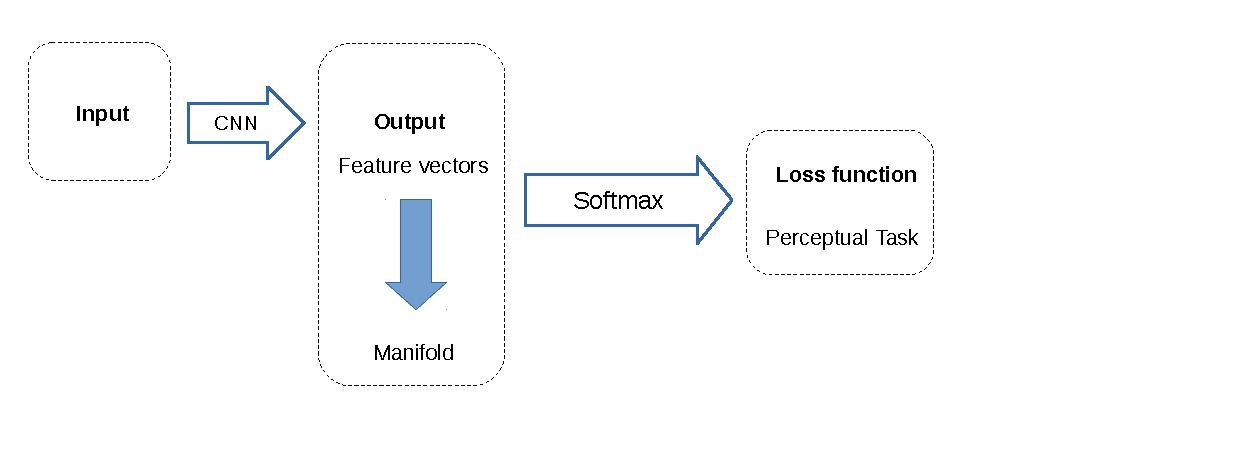
\includegraphics[width=0.9\textwidth]{img/model2}}


\subsection*{Proposed criterion}

If we introduce the manifold dimension as a regularizer, we can write after \cite{zhu2017ldmnet}:
\[ \min_{{\bf w}, {\cal M}} \; (1 - \mu) \, {\cal L}({\bf w}) + \mu \frac{\int_{\cal M} d {\bf p} \; \left.dim({\cal M})\right|_{\bf p}}{\int_{\cal M} d {\bf p} \; 1}, \mbox{ with } {\bf f}_{\bf w}({\bf i}_n) \in {\cal M}  \subset {\cal R}^D\] 
i.e. the average dimension, averaged by the volume $vol({\cal M}) = \int_{\cal M} d {\bf p} \; 1$. Here $\mu \in [0, 1]$ allows to balance the regularization.

This idea has been originaly applied in computer vision \cite{osher2017low}, includinf e-paiting \cite{zhu2017nonlocal} and scientific data interpolation \cite{zhu2018scientific}.

The manifold is locally parameterized by coordinate functions $\psi(\cdot)$:
\eqline{\psi: {\bf q} \in U \subset {\cal R}^d \rightarrow {\bf p} \in {\cal M} \subset {\cal R}^D}
These coordinates function ideally correspond to the computation output ${\bf f}_{\bf w}(\cdot)$. Adjusting the manifold ${\cal M}$ means adjusting these coordination functions $\psi(\cdot)$ in order to reduce the average dimension. Furthermore, from  \cite{zhu2017nonlocal} (see Appendix~\ref{manifold}):
\eqline{\int_{\cal M} d {\bf p} \; \left.dim({\cal M})\right|_{\bf p} = \sum_{j=1}^D \int_{\cal M} d {\bf p} \; \|\nabla \psi^j\|^2}
since the sum of the squared norm of the coordinate function gradient precisely corresponds to the local dimension (see Appendix~\ref{manifold}).

\subsubsection*{Manifold regularization}

With this result, the criterion is close to usual manifold regularization \cite{belkin2006manifold}, requiring the input-output map itself to be a smooth function, in the sense of changing slowly on the data manifold, i.e., on where the input data is dense, i.e.:
\eqline{\min_{{\bf w}} \; {\cal L}({\bf w}) + \mu' \int_{\cal M} {\bf p} \; P({\bf p}) \, \|\nabla {\bf f}_{\bf w}\|^2}
writing $\mu = \mu' \, vol({\cal M})$. Here $P({\bf p})$ stands for the data probability density while $P(p) \equiv 1$ since the sampling is assumed to be uniform. Since in the ideal case $\psi(\cdot) = {\bf f}_{\bf w}(\cdot)$, both criteria correspond. They are however not minimized the same way.

\well{@Wei Is this exact, or do i miss something ?}

Similarly this criterion can be related to \cite{mukherjee2010learning} learning gradients on manifolds for dimension reduction for high-dimensional data with few observations. The authors obtain generalization error bounds for the gradient estimates and show that the convergence rate depends on the intrinsic dimension of the manifold and not on the dimension of the ambient space.


\subsubsection*{Discretized criterion}

Here, we consider perturbed coordinate functions, and will not only adjust the input-output computation parameters ${\bf w}$, but also the manifold itself, parameterized by the coordinate functions.

The original method further separate the minimization with respect to weights ${\bf w}$ calculation, from the manifold parameterization optimization (using alternating direction method of multipliers), compute the Euler-Lagrange equation in the continuous formalism and then discretize the resulting Laplace-Beltrami operator, via a point integral method, in order to derive a tractable algorithm.

We may also consider a direct discretization of the gradient, instead. Considering the discrete set of data point the standard method to discretize an integral is to:
\\- Identify the neighbors of each data point ${\bf o}_n$. This can be done by finding the k-nearest neighbors, or by choosing all points within some fixed radius $\rho$ in ${\cal R}^D$.
\\- Choose a local kernel $R({\bf p}, {\bf p}')$ (see Appendix~\ref{integral}) allowing to approximate the gradient by finite difference, i.e., to write:
\[ \sum_{j=1}^D \int_{\cal M} d {\bf p} \; \|\nabla \psi^j\|^2 
\simeq \int_{\cal M} d {\bf p} \int_{\cal M} d {{\bf p}'} \; R({\bf p}, {\bf p}') \, \|\psi({\bf p}) - \psi({\bf p}')\|^2
\simeq \sum_{n,n'} R({\bf o}_n, {\bf o}_{n'}) \, \|{\bf o}_n - {\bf o}_{n'}\|^2 \]

The left-hand size approximation is directly related to point integral method since by the Stroke's theorem gradient and Laplacian are linked, as reviewed in Appendix~\ref{integral}. The right-hand size approximation is a simple sampling. 

\well{@Wei Looks ``too simple'' is something wrong proceeding that way ?}

\subsubsection*{Criterion minimization}

Merging these elements we are left with the variational problem:
\[  \min_{{\bf w}, {\bf \psi}} \; {\cal C},\; {\cal C} \deq (1 - \mu) \, {\cal L}({\bf w}) + \mu \, \sum_{n,n'} R_{nn'} \, \|{\bf \psi}_n -  {\bf \psi}_{n'}\|^2 + \sum_n \lambda_n \, ({\bf o}_n - {\bf \psi}_n) + \gamma \, \|{\bf o}_n - {\bf \psi}_n\|^2\]
where ${\bf o}_n = {\bf f}_{\bf w}({\bf i}_n)$, we write $R_{nn'} \deq R({\bf o}_n, {\bf o}_{n'})$, ${\bf \psi}_n$ is a perturbed value of ${\bf o}_n$ which tends to reduce the dimension and $\lambda_n$ are Lagrange multipliers while the term with $\gamma$ introduces a augmented Lagragian mechanism. Being in a discrete set-up allows us to derive basic normal equations:
\[ \begin{array}{rcl}
 \nabla_{\bf w} {\cal C} &=& \nabla_{\bf w} {\cal L}({\bf w}) + \sum_n (\lambda_n + 2 \, \gamma \, ({\bf o}_n - {\bf \psi}_n))\, \nabla_{\bf w} {\bf f}_{\bf w}({\bf i}_n) \\
0 = \nabla_{{\bf \psi}_n} {\cal C}^T &=& \mu \, 2 \sum_{nn'} (R_{nn'} + R_{n'n}) \, ({\bf \psi}_n - {\bf \psi}_{n'}) - \lambda_n + 2 \, \gamma \, ({\bf \psi}_n - {\bf o}_n) \\
0 = \nabla_{{\bf \lambda}_n} {\cal C}^T &=& {\bf o}_n - {\bf \psi}_n \\
\end{array} \]

{\em Direct minimization} When eliminating ${\bf \psi}$ (thus ${\bf \lambda}$ and $\gamma$) we obtain the following modified minimization gradient:
\eqline{\nabla_{\bf w} {\cal C} = \nabla_{\bf w} {\cal L}({\bf w}) + 2 \, \mu \, \sum_{nn'} (R_{nn'} + R_{n'n}) \, ({\bf o}_n - {\bf o}_{n'}) \, \nabla_{\bf w} {\bf f}_{\bf w}({\bf i}_n).} According to \cite{zhu2017nonlocal}, the drawback of this simple approach is that the optimization problem is highly nonlinear and nonconvex, and we thus may get stuck in a local minimum.

{\em Alternating minimization} If we maintain a alternating minimization, the equation $0 = \nabla_{{\bf \psi}_n} {\cal C}^T$ provides, given $\gamma$ and $\lambda$, linear equations in ${\bf \psi}$, while the modified minimization gradient is given by $\nabla_{\bf w} {\cal C}$. In that case the minimization may start with ${\bf \lambda} = 0$, $\gamma = \mu$ and when a minimum is obtained 
\eqline{{\bf \lambda}_n^{t+1} \leftarrow  {\bf \lambda}_n^{t} + \gamma^{t} \, ({\bf o}_n - {\bf \psi}_n), \gamma^{t+1} \leftarrow \left\{ \begin{array}{ll}
\gamma^{t} & \mbox{ if $\|{\bf o}_n - {\bf \psi}_n\|^2$ decreases} \\ 2\, \gamma^{t} & \mbox{ otherwise } \\ \end{array}\right.}
This completely specify the algorithmic hyper-parameters.

\well{@Wei I understand that ADMM allows to ``convexify'' the criterion, but since ${\cal L}(\cdot)$ is not, why should we gain something with respect to direct gradient minimization ?}

\subsubsection*{Initialization and hyper-parameter adjustment.}

We may start considering the manifold as the union of 0-dimensional manifolds, i.e., prototypes, thus start by a k-mean clustering. This provides us with an initial value of $\sum_{n,n'} R_{nn'} \, \|{\bf \psi}_n -  {\bf \psi}_{n'}\|^2$, likely maximal since we choose here a solution with a minimal number of degree of freedom, with respect to a more general manifold representation. 

Performing the minimization with $\mu = 0$ (i.e., without regularization) provides us with a minimal value of ${\cal L}(\cdot)$ on the learning set (not on the cross-validation) since we expect over-fitting, that is going to be avoided by regularization.

We then can explore values of $\mu \in [0, 1]$ and choose the best meta-learning result.

\appendix \clearpage

\section{Manifold notation}\label{manifold}

The manifold is locally parameterized by:
\eqline{\psi: {\bf q} \in U \subset {\cal R}^d \rightarrow {\bf p} \in {\cal M} \subset {\cal R}^D}
thus ${\bf p} = \psi({\bf q})$, i.e., in coordinates, $p^j = \psi^j((\cdots q^i \cdots)^T), i \in \{1, d\}, j \in \{1, D\}$, while $d = \left.dim({\cal M})\right|_{\bf p}$ at the point ${\bf p}$. The point ${\bf p}$ is represented by $D$ coordinates, subject to $D - d$ constraints. We writes $\partial_i^j = \frac{\partial \psi^j({\bf q})}{\partial q^i}$.

At each point the tangent space is a $d$-dimensional linear space $T_{\bf p}{\cal M}$, equipped with an inner product written $<\cdot, \cdot>$.

Between two points ${\bf p}, {\bf p}' \in {\cal M}$ there is a notion of distance induced by a minimal length path, called geodesic. Locally, we can map a point ${\bf p}$ onto a point ${\bf p}'$ along a geodesic given an infinitesimal displacement along a vector ${\bf v}$ of the tangent space (notion of ``exponential'' map).

In order to define the required quantities, let us use the implicit summation convention in conjunction with the Kronecker symbol:
~
\\- The covariant tangent vector along a direction $q^i$, writes $\partial_i = (\cdots \partial_i^j \cdots)^T$.
\\- The metric tensor writes $g_{ii'} = <\partial_i, \partial_{i'}> = \delta_{jj'} \, \partial_i^j \, \partial_i^{j'}$.
\\- Its inverse writes $g^{i'i''} = \partial^{i'} \partial^{i''}$, with $g_{ii'} \, g^{i'i''} = \delta_i^{i''}$.
\\- The gradient of a function $f$ writes: $\nabla f = f^i \, \partial_i = g^{ii'} \, \partial_{i'} f \, \partial_i$.
\\- The differential of a function $f$ writes: $d f $, with $d f(X) = \partial_i f \, X^i = <\nabla f, X>$, i.e., in matrix form: $\nabla f = g^{-1} df$.

See \cite{lee2003smooth} for a complete introduction on smooth manifold and \cite{gudmundsson2008introduction} for an introduction on Riemannian geometry.



\subsection*{A few derivations}

We can relate $f^i$ to $\partial_{i} f$ by the following derivation:
\eqline{\partial_{i} f = df(\partial_{i}) = <\nabla f, \partial_{i}> = <f^{i'} \, \partial_{i'}, \partial_{i}> = f^{i'} \, <\partial_{i'}, \partial_{i}> = f^{i'} \, g_{i'i}}
and in the reverse:
\eqline{g^{ii'} \, \partial_{i'} f = g^{ii'} \, f^{i''} \, g_{i''i'} = f^{i''} \,  g^{ii'} \, g_{i''i'} = f^{i''} \, \delta_{ii''} = f^i}
considering that $g$ is symmetric.

We these notations, we easily derive after \cite{zhu2018scientific}:
\eqline{\begin{array}{rcl} \sum_{j=1}^D \|\nabla \psi^j\|^2 
&=& \delta_{jj'} \, (g^{ii'} \, \partial_{i'} \psi^j \, \partial_i) \, (g^{i''i'''} \, \partial_{i'''} \psi^{j'} \, \partial_{i''}) \\
&=& (g^{ii'} \, \partial_i) \, (g^{i''i'''} \, \partial_{i''}) \, (\delta_{jj'} \, \partial_{i'} \psi^j \, \partial_{i'''} \psi^{j'})   \\
&=& (g^{ii'} \, \partial_i) \, (g^{i''i'''} \, \partial_{i''}) \, g_{i'i'''} \\
&=& (\partial^{i'} \, \partial^{i''}) \, g_{i'i'''} \\
&=& g^{i'i'''} \, g_{i'i'''} = \delta_{i'}^{i'} = d \\
\end{array}}

\section{Integral approximation of gradient norm} \label{integral}

The goal is to derive:
\[ \sum_{j=1}^D \int_{\cal M} d {\bf p} \; \|\nabla \psi^j\|^2 
\simeq \int_{\cal M} d {\bf p} \int_{\cal M} d {{\bf p}'} \; R({\bf p}, {\bf p}') \, \|\psi({\bf p}) - \psi({\bf p}')\|^2 \]

Following \cite{li2017point}, we use the Taylor expansion:
\eqline{f({\bf p}) - f({\bf p}') = ({\bf p} - {\bf p}') \nabla f({\bf p}) + O(\|{\bf p} - {\bf p}'\|^2)}
and the fact that for a local kernel such as $R({\bf p}, {\bf p}') = \nu \, e^{-\frac{\|{\bf p} - {\bf p}'\|^2}{\rho^2}}$
\eqline{\int_{\cal M} d {\bf p} R({\bf p}, {\bf p}')\, \|{\bf p} - {\bf p}'\|^n = O(\rho^n)}
while from the Stroke theorem:
\eqline{\int_{\cal M} d {\bf p} \; \|\nabla f({\bf p})\|^2 = \int_{\cal M} d {\bf p} \; f({\bf p})\, \Delta f({\bf p})}

\well{@vthierry To be done, this seems to be no more than a variant of usual PIM}

{\scriptsize \bibliographystyle{alpha}\bibliography{../bib/vthierry}}\end{document}


